%% *************************************************************************
%%
%% This is an RIT Space Exploration Standard defining guidelines for content
%% and formatting of project design documents.
%%
%% This document uses IEEEtran.cls, the official IEEE LaTeX class
%% for authors of the Institute of Electrical and Electronics Engineers
%% (IEEE) Transactions journals and conferences.
%%
%% *************************************************************************

%% *************************************************************************
% LaTeX REFERENCES
% ----------------
%   Intro to LaTeX: http://www.rpi.edu/dept/arc/docs/latex/latex-intro.pdf
%   Comprehensive LaTeX symbol list: http://tug.ctan.org/info/symbols/comprehensive/symbols-a4.pdf
%% *************************************************************************

% tell \LaTeX what kind of formatting to use
\documentclass[conference]{IEEEtran} % http://www.ctan.org/pkg/ieeetran
% enable placeholder text generator
\usepackage{blindtext}
% enable toolbox for embedding figures and pictures
\usepackage{graphicx}
% enable package for adding a list of variables and constants at the beginning, aka "nomenclature"
\usepackage{nomencl}
% enable package for easily formatting units
\usepackage{siunitx}
% enable package for cross-referencing figures, sections, references etc.
% how to use hyperref: http://www2.washjeff.edu/users/rhigginbottom/latex/resources/lecture09.pdf
\usepackage{hyperref}
% change text encoding to make it more crisp
\usepackage[T1]{fontenc}
% enable conditionals for help text
\usepackage{etoolbox}
% initialize nomenclature packageDecember
\makenomenclature{}


%%% Non-PDD-Template Use Packages %%%
% enable subfigures
\usepackage{subcaption}
% enable PDF import
\usepackage{pdfpages}

\title{Design of an Aerospike Nozzle}

\author{
	% List the authors of the design document. The Champion should go first.
	% The \$~\$ markers tell \LaTeX{} to treat the text inside to be treated as a math expression. This way you can use operators like \textcaret{} to place characters as superscripts.
	% Some \LaTeX{} templates handle the author block in different ways. For example, the \href{http://www.worldscientific.com/worldscinet/jai}{Journal of Astronomical Instrumentation} requires the authors' addresses and emails to be included as well.
	% The \textbackslash{}thanks command puts the contents inside those brackets in a footnote at the bottom of the first page. Technically speaking, \textbackslash{}thanks is just a specially formatted footnote.
	% IEEE also has a ``long form'' author block for many authors. Check here for more information:
	% \url{https://tex.stackexchange.com/questions/156523/multiple-authors-with-common-affiliations-in-ieeetran-conference-template}
	% Read here for a more advanced options to modifying footnotes in the author block:  \url{http://tex.stackexchange.com/questions/826/symbols-instead-of-numbers-as-footnote-markers}
	%   Here, we use the IEEE long-form author block.
	\IEEEauthorblockN{% This block is for author Names.
		Hunter~Collins\IEEEauthorrefmark{1},  %the number in the bracket is a reference number to identify this footnote. \LaTeX will figure out what symbol to put there.
	}
	\IEEEauthorblockA{% This block is for the author Affiliations, aka department and university
		RIT Space Exploration, Rochester Institute of Technology \\ %\\ starts a new line
		Rochester, N.Y. \\
		Email:
		\IEEEauthorrefmark{1}hwc8092@rit.edu
	}
	%%   Below, we use the short-form author block and basically hack it to suit our needs.
	% Philip~Linden$^{*\dagger}$%
	%   \thanks{$^{*}$Project Champion}%
	%   \thanks{$^{\dagger}$BS/MEng '17, Mechanical Engineering},
	% Austin~Bodzas$^{\ddagger}$%
	%   \thanks{$^{\ddagger}$BS '19, Computer Science},
	% Drew~Walters$^{\S}$%
	%   \thanks{$^{\S}$BS '18, Mechanical Engineering Technology},
	% T.J.~Tarazevits$^{**}$%
	%   \thanks{$^{**}$BS '19, Game Design \& Development}%
	
	%%   If there are many authors, consider using symbolic, numeric (aka arabic),  alphabet footnotes or a combination thereof.
	%% the recommended order for symbolic footnotes is
	%%   (1) asterisk        *   *
	%%   (2) dagger          †   \dagger
	%%   (3) double dagger   ‡   \ddagger
	%%   (4) section symbol  §   \S
	%%   et cetera. For higher counts, use 2x symbols (1)-(4) (i.e. (5) two asterisks **). Keep cycling through (1)-(4) using 3x, 4x, and so on.
	%%   Note that these symbol codes work in math mode and text mode.
	%%   There are ways to make LaTeX do this for you, but it is more advanced and not entirely necessary, especially for short author lists. Not worth the hassle, in my opinion.
}
% page header for pages other than cover page
\markboth{Project Design Document Standard}%
{Collins \MakeLowercase{\textit{et al.}}: RIT Space Exploration}

% Initial setup is over, start building the document itself
\begin{document}
	\maketitle%
	% correct bad hyphenation here, separated by spaces
	\hyphenation{explor-ation}
	
	\begin{abstract}
		Historically, spaceflight has been prohibitively expensive. If engineers are going to pave the way for increased access to space, they must seek out novel propulsion technologies rather than continually improving upon existing technology. The aerospike nozzle, while not a new concept, has a lack of flight heritage and been repeatedly predicted to outperform a conventional bell nozzle's thrust efficiency due to its altitude-compensating exhaust flow. This project will conduct cold flow experiments, develop nozzle design software, and design an aerospike nozzle to propel a sounding rocket to 100 km. The data and knowledge gained from this project will be collected and published in an effort to increase the aerospike nozzle's flight-readiness level for academic, governmental, and commercial launch vehicles alike.
	\end{abstract}
	
	\label{sec:nomenclature}
	\newcommand{\nomunit}[1]{%
		\renewcommand{\nomentryend}{\hspace*{\fill}#1}}
	\renewcommand{\nompreamble}{
		% If you include mathematical expressions or express variables in the design document, list them with their corresponding definitions here as a list.
		% The two lines below make it look nice when defining units/values to constants.
		
		% Note that math terms and non-math terms are separated and alphabetized, regardless of the order in which they are defined. (Recall terms \$like this\$ are in the math environment)
		% Read more about advanced nomenclature formatting here:\\
		% \url{https://www.sharelatex.com/learn/Nomenclatures}
	}
	\nomenclature{SPEX}{RIT Space Exploration}
	\nomenclature{CBN}{conventional bell nozzle}
	\nomenclature{AIAA}{American Insitutde of Aeronautics \& Astronautics}
	\nomenclature{CAD}{computer-aided design}
	\nomenclature{CFD}{computational fluid dynamics}
	\nomenclature{FEA}{finite element analysis}
	\nomenclature{DAQ}{data aquisition}
	\nomenclature{(\textit{Fig. symbols, ETC.})}{\textit{(Will be including them.)}}
	
	% Below are examples of using nomenclature for math symbols and constants or units
	% \nomenclature{$\dot{m}$}{Mass flow rate
	%   \nomunit{\,\si{\kilo\gram\per\second}}}
	% \nomenclature{$c$}{Speed of light
	%  \nomunit{\,\SI{2.9979e8}{\meter\per\second}}}
	\printnomenclature{}
	
	% HELPFUL HINT: If you get the warning ``Command terminated with space.'' when using a \command try placing ``%'' or ``{}'' immediately following the command.
	
	\section{Introduction}
	\label{sec:introduction}
	% The introduction is a place to give background and context before diving into the subject matter.
	% Establish context for the work you are about to propose and the main ideas of the proposition itself.
	
	\IEEEPARstart{S}{paceflight} is expensive. With the rising demand for low-cost satellite and microsatellite launches and the recent growth in the commercial spaceflight industry \cite{FAAAeroForecast2016, AlJazeeraSpaceArticle}, minimizing the cost per pound to the common satellite destinations of low Earth orbit and geostationary orbit has never been more critical \cite{LA-Times_InvestmentInSpace}.
	
	The efficiency of a launch vehicle has a significant impact on the overall cost of mission. Therefore, alternative engine designs have been researched in pursuit of the optimal propulsion system. The aerospike nozzle (see Figure \ref{fig:aerospike}) is among the most prominent of alternative nozzle designs as it possesses an altitude-compensating ability. All conventional bell nozzles (CBN) perform optimally at a specific ambient pressure for a given throttle level (or chamber pressure). The corresponding altitude for this ambient pressure is referred to as the `design altitude'. Thus, at all other altitudes the nozzle strays from performing optimally. While susceptible to the very mechanism by which the CBN loses its efficiency (that is, divergence loss), the aerospike nozzle has a notable efficiency advantage shown in Figures \ref{fig:1} through \ref{fig:3}. For the readers' convenience, a more detailed explanation of this phenomena is provided in Appendix B.
	
	\begin{figure}
		\centering
		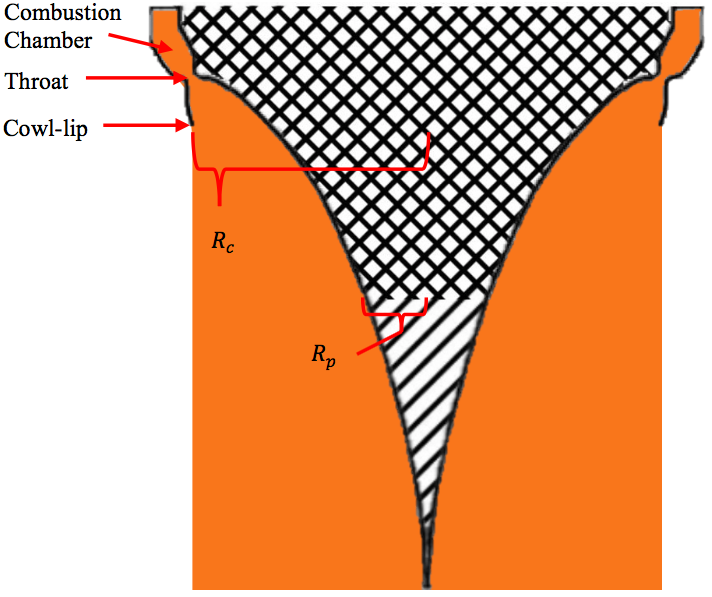
\includegraphics[width=0.75\columnwidth]{figs/aerospike.png}
		\caption{Diagram of aerospike nozzle operating at its design altitude, depicting various components and area dimensions. Excluding the spike segment toward the bottom (filled with a diagonal pattern) would result in a plug nozzle configuration.}
		\label{fig:aerospike}
	\end{figure}
	
	\begin{figure}
		\centering
		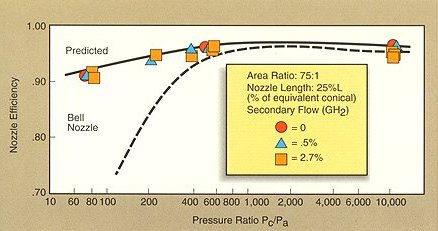
\includegraphics[width=\columnwidth]{figs/ASvsCBN_NozzleDesign.jpg}
		\caption{Nozzle Efficiency vs. Pressure Ratio. Top and bottom line represent predicted aerospike and bell nozzle efficiency, respectively}
		\label{fig:1}
	\end{figure}
	
	\begin{figure}
		\centering
		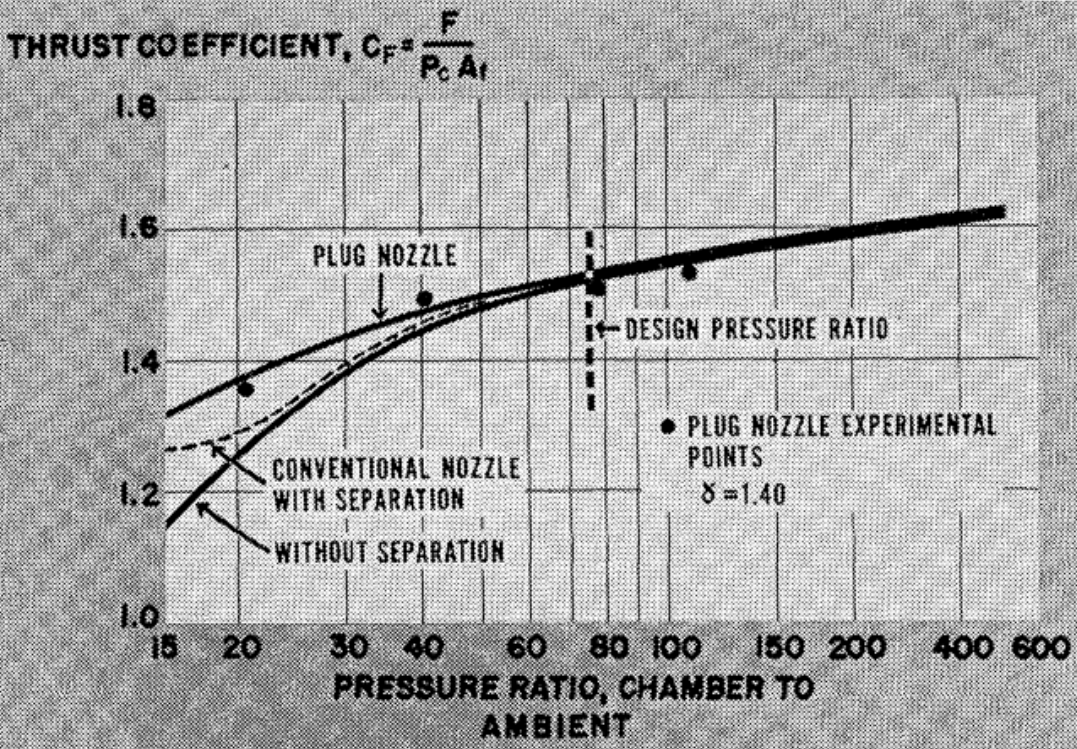
\includegraphics[width=\columnwidth]{figs/GraphOfASPerformance_Rao.png}
		\caption{Thrust Coefficient vs. Pressure Ratio.}
		\label{fig:2}
	\end{figure}
	
	\begin{figure}
		\centering
		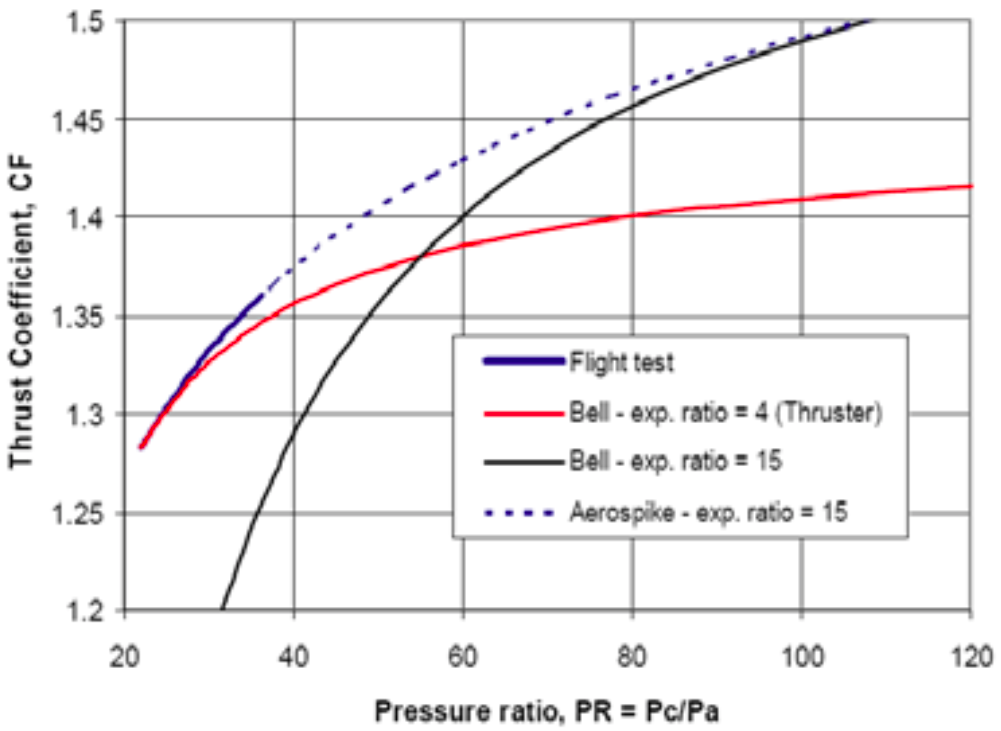
\includegraphics[width=\columnwidth]{figs/CALVEIN's_AS_CFD_analysis.png}
		\caption{Thrust Coefficient vs. Pressure Ratio. Includes flight test data points and predictions which follow computer simulation data.}
		\label{fig:3}
	\end{figure}
	
	\section{Primary Objective}
	\label{sec:primary-obj}
	% At the end of the day, whether the project ``succeeds'' or ``fails'' is judged against the objectives it sought to meet.
	% Note that results that contradict expectations/hypotheses are not failures if the scientific \& engineering methods are followed along the way.
	% Sometimes our expectations are wrong and that can be just as successful as getting data we thought we'd see.
	% What matters are what questions you intend to answer.
	% This is the main purpose or main goal the project hopes to achieve.
	
	The primary objective of this project is to further characterize flow of aerospike nozzles by building upon current simulation methods and models through mathematical analysis and physical validation (i.e. cold flow experiments). This experience and knowledge will concurrently be applied to the design on an aerospike nozzle to propel a sounding rocket to 100 km. 
	
	
	% \section{Secondary Objectives}
	% \label{sec:secondary-obj}
	% Secondary Objectives are lower priority or bonus objectives that are significant but not the main focus of the project. This template does not have secondary objectives.
	
	\section{Benefit to SPEX}
	\label{sec:benefit}
	% One of the core values of SPEX is to provide opportunities for academic and professional growth for its members,
	% and to challenge them with interesting projects.
	% In this section, explain how the project would benefit SPEX members as students,
	% space enthusiasts, and young professionals.
	
	Members of SPEX who are involved in this project will acquire a host of technical skills related to simulation, modeling, programming, design engineering, data acquisition, and experimental analysis. These skills will play a critical role in future SPEX Propulsion projects as well as SPEX-wide endeavors as well, such as the NASA CubeSat Launch Initiative. Employers are in-search of those with experience in analysis, physical validation, and how the iterative relationship between them can yield a better end-product.
	
	Additionally, this project's findings will be thoroughly documented, culminating in a paper, presentation, and poster to exhibit at events such as the Undergraduate Research Symposium, ImagineRIT, and an AIAA technical conference. Attending these events and presenting our published work will help establish SPEX in the science and aerospace communities.
	
	\section{Implementation}
	\label{sec:implementation}
	
	This project is expected to take two semesters. The first semester will be devoted to developing the MATLAB script and running simulations. Initial cold flow test results from \textit{Investigation of a Cold Gas Thruster}\cite{coldgaspdd} will help validate values outputted by scripts and simulations, as related to CBNs. From there, CFD will be used to validate the MATLAB script when aerospike nozzle contouring is undertaken. The first semestester will also include the mechanical design of the aerospike nozzle and the low pressure chamber used to simulate ascent through the atmosphere. During this physical simulation, we will be able to observe how the exhaust plume changes with respect to ambient pressure and thrust data points.
	
	\subsection{Deliverables}
	\label{subsec:deliverables}
	Software:
	\begin{itemize}
		\item \textit{Nozzle Design and Modeling Tool} MATLAB script
		\begin{itemize}
			\item  Design equations for CBN and aerospike:
			\begin{itemize}
				\item Isentropic
				\item Method of Characteristics
			\end{itemize}
			\item  Efficiency losses:
			\begin{itemize}
				\item Thrust efficiency at designated altitudes
				\item Cumulated (thrust) efficiency loss over duration of vehicle's flight path
				\item 3 main CBN nozzle efficiency losses
				\item Efficiency losses from a constant external fluid flow
			\end{itemize}
		\end{itemize}
		\item CFD, FEA
		\begin{itemize}
			\item Computer simulations will be used to reduce number of designs to experimentally test. They will also serve to improve and validate MATLAB scripts and CAD designs.
		\end{itemize}
	\end{itemize}
	Hardware:
	\begin{itemize}
		\item Machined nozzles (smooth-walled)
		\item Low pressure chamber addition to cold flow test stand
		\item Apparatus to observe and measure external fluid flow around aerospike
		\item DAQ system
	\end{itemize}
	Events:
	\begin{itemize}
		\item Undergraduate Research Symposium
		\begin{itemize}
			\item Detailed poster
			\item Cold flow test stand on display
		\end{itemize}
		\item ImagineRIT
		\begin{itemize}
			\item Overview poster
			\item Cold flow test stand on display
		\end{itemize}
		\item AIAA Technical Conference
		\begin{itemize}
			\item Detailed poster
			\item Presentation
		\end{itemize}
	\end{itemize}
	Publications:
	\begin{itemize}
		\item Monthly SPEX Wiki updates
		\item Technical paper published in AIAA technical conference format
	\end{itemize}
	
	\subsection{Milestones}
	\label{subsec:milestones}
	\textit{(Should I just reference the draft gaant chart found in Appendix A?)}
	
	\section{Externalities}
	% Things not directly related to the work or outcomes, but related to the project as a whole.
	\subsection{Prerequisite Skills}
	An overall understanding of compressible flow. Previous experience with MATLAB among at least three of the project members is required. At least one project member must have experience using electronics and sensors.
	
	\subsection{Funding Requirements}
	Excluding CFD and FEA license(s), the cost of all raw materials and DAQ instruments will likely cost \$400 to \$600. If everything is purchased and not donated/sponsored, the most expensive cost would likely be CFD and/or FEA license(s). Fortunately, there have been companies in the past who have donated software licenses, materials, and other equipment to RIT extracurricular groups.
	
	\subsection{Faculty Support}
	Faculty guidance may be needed to help explain some of the concepts this project will explore (e.g. compressible fluid flow, shocks). Guidance may also be needed with DAQ. \textit{(Should specific faculty be listed?)}
	
	\subsection{Long-Term Vision}
	\label{sec:vision}
	Cultivating an environment that inspires ingenuity is an essential part to SPEX's mission. The predicted efficiency improvement of an aerospike nozzle, combined with its lack of flight heritage, makes it an exciting avenue for research. During this project, the additions made to the cold flow test stand and code written will provide the base for which future nozzle's may be tested and designed using, respectively.
	
	\section*{Acknowledgements}
	The author would like to thank Dr.~Bill Destler and Rebecca Johnson for being exemplary humans, Anthony Hennig for founding RIT Space Exploration, and all the SPEX members that continue to invest their time and energy in (\textit{into} replaced with \textit{in}) the pursuit of space exploration.
	
	\bibliographystyle{IEEEtran}
	\bibliography{myrefs}
	
	\onecolumn
	
	\appendices{}
	
	\section{Aerospike Nozzle: Advantages \& Complications}
	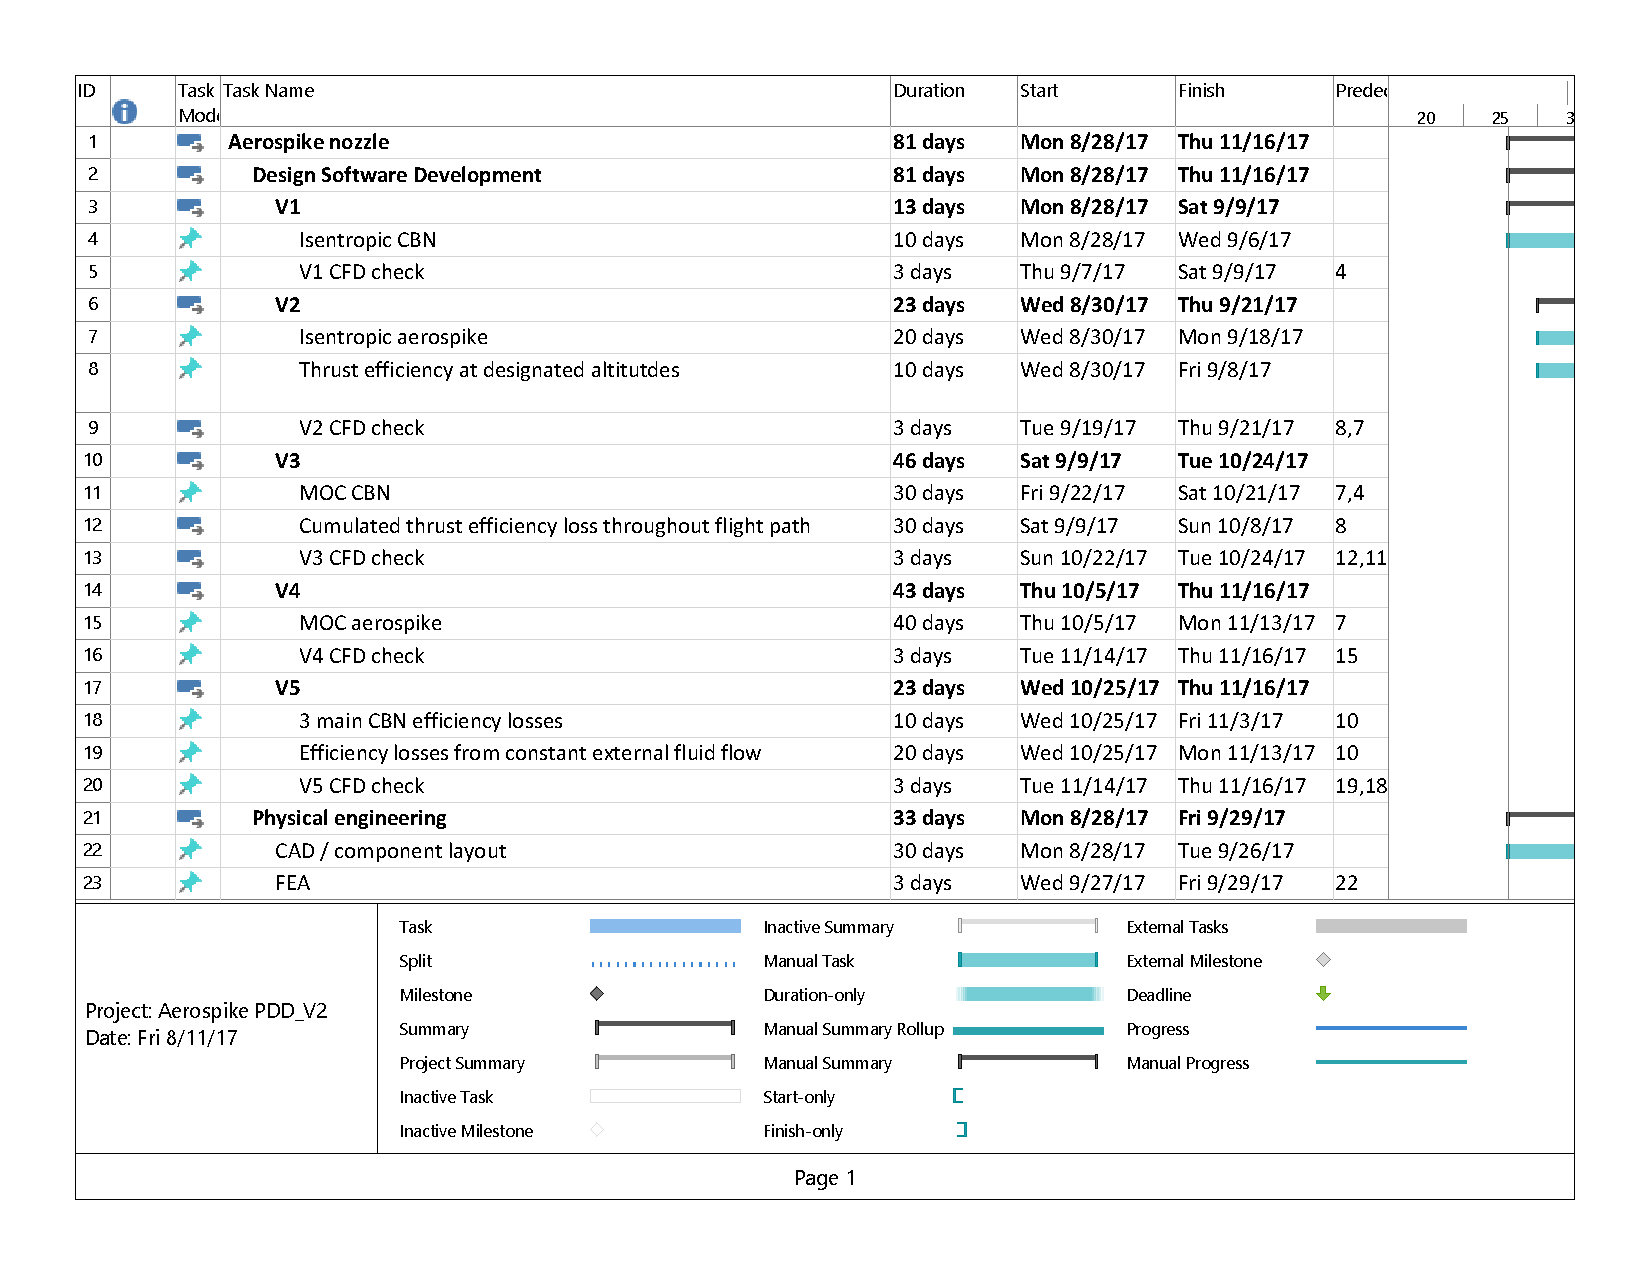
\includepdf[pages={1-},scale=1, landscape=true]{figs/V2_Aerospike.pdf}
	%	\label{}
	
	\section{Draft Project Plan (Aerospike Project Plan V2)}
	\includepdf[pages={1-},scale=1]{figs/V4_AerospikeNozzle.pdf}
	%	\label{}
	
\end{document}